\documentclass[hyperref={pdfpagelabel=false},usepdftitle=false,xcolor=dvipsnames]{beamer}

\usepackage[T1]{fontenc}
\usepackage[utf8]{inputenc}
\usepackage[russian]{babel}

\usepackage{amssymb, amsmath}

% table/tabular packages
\usepackage{tabularx, rotating, ragged2e, booktabs, caption}
\usepackage{graphicx}
\usepackage[verbose]{placeins}
\usepackage{blindtext}
\usepackage{multicol}

\usetheme{CambridgeUS}
\useinnertheme{rectangles}
\useoutertheme{infolines}

\newcommand\Fontvi{\fontsize{6}{7.2}\selectfont}

\beamertemplatenavigationsymbolsempty

\setbeamerfont{page number in head/foot}{size=\large}
\setbeamertemplate{footline}[frame number]
\setbeamertemplate{frametitle}[default][center]

% change font
\usefonttheme[onlymath]{serif}

\makeatother
\setbeamertemplate{headline}
{}
\makeatletter

% adding roman numerals
\makeatletter
\newcommand*{\rom}[1]{\expandafter\@slowromancap\romannumeral #1@}
\makeatother
\usepackage{makecell}
\newcolumntype{x}[1]{>{\centering\arraybackslash}p{#1}}
\usepackage{tikz}
\newcommand\diag[4]{%
  \multicolumn{1}{p{#2}|}{\hskip-\tabcolsep
  $\vcenter{\begin{tikzpicture}[baseline=0,anchor=south west,inner sep=#1]
  \path[use as bounding box] (0,0) rectangle (#2+2\tabcolsep,\baselineskip);
  \node[minimum width={#2+2\tabcolsep-\pgflinewidth},
        minimum  height=\baselineskip+\extrarowheight-\pgflinewidth] (box) {};
  \draw[line cap=round] (box.north west) -- (box.south east);
  \node[anchor=south west] at (box.south west) {#3};
  \node[anchor=north east] at (box.north east) {#4};
 \end{tikzpicture}}$\hskip-\tabcolsep}}



\usepackage{graphicx}

\begin{document}

\begin{frame}{\normalsize Поверхности потенциальной энергии межмолекулярного взаимодействия \rom{1}}
\begin{figure}
\vspace*{-0.3cm}
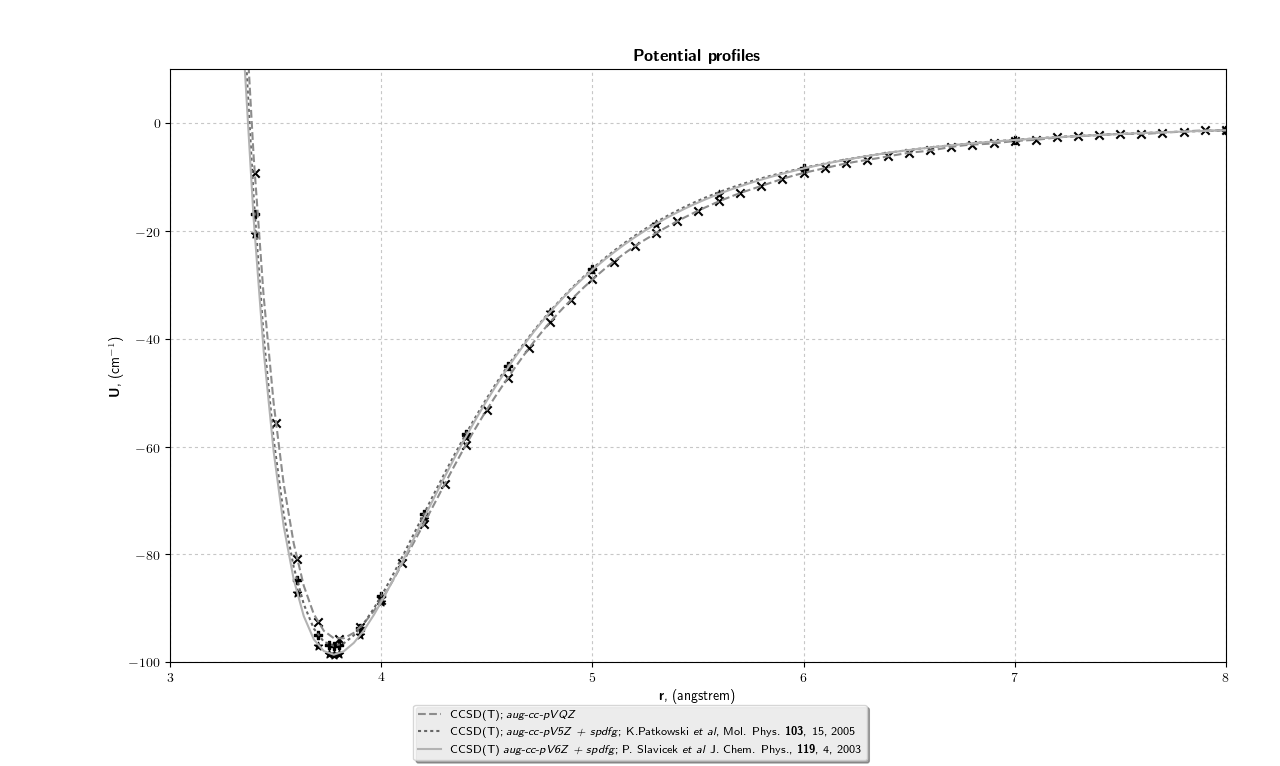
\includegraphics[width = \linewidth]{pictures/pp38.png}
\end{figure}
\end{frame}

\begin{frame}{\normalsize Поверхности потенциальной энергии межмолекулярного взаимодействия \rom{2}}
\begin{figure}
\vspace*{-0.3cm}
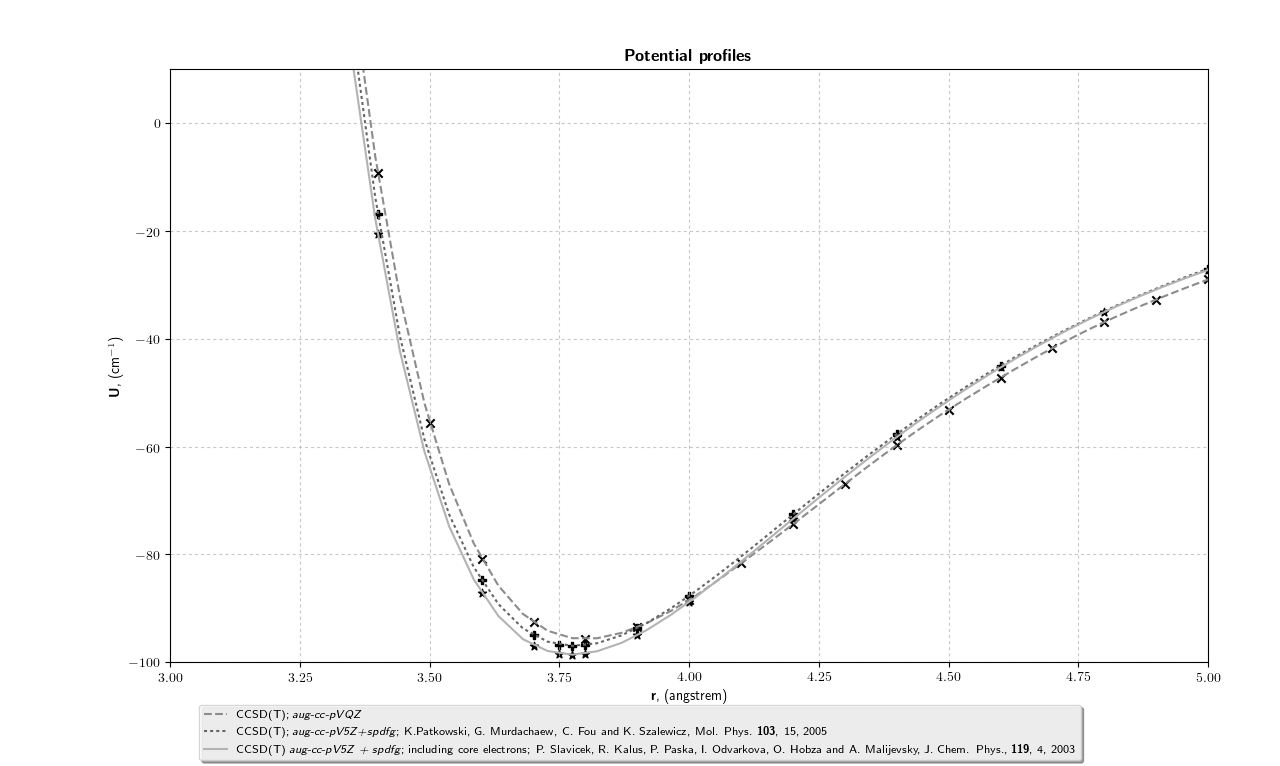
\includegraphics[width = \linewidth]{pictures/pp35.png}
\end{figure}
\end{frame}

\begin{frame}{\normalsize BSSE}
\captionof{table}{Mol. \& vib. params. $H_2 O$}
\begin{tabular}{ccccc}
\toprule
& \multicolumn{2}{c}{Values} & \multicolumn{2}{c}{Freqs} \\
\cmidrule(r){2-3} \cmidrule(r){4-5}  
& Calc. & Exp. & Calc. & Exp. \\
\cmidrule(r){2-3} \cmidrule(r){4-5}
r(O-H) & 0.965 & $0.958$ & $3931$ & 3657 (asym.) \\
$\angle$ HOH & $105.754$ & $104.478$ & $3809$ & 3756 (sym.) \\
$\mu$ (D) & 2.195 & $1.855$ & $1603$ & $1595$ \\
	       & B3LYP; 6-31+G** & NIST & B3LYP; 6-31+G** & NIST \\
\bottomrule
\end{tabular}
\end{frame}


\end{document}

